%----------------------------------------------------------------
%
%  File    :  vpn_setup.tex
%
%  Author  :  Keith Andrews, IICM, TU Graz, Austria
% 
%  Created :  22 Feb 96
% 
%  Changed :  19 Feb 2004
% 
%----------------------------------------------------------------

\chapter{Environment Setup} \label{chap:Setup}

This chapter provides an in-depth discussion of the environment used for both learning and fuzzing, focusing on its setup and configuration. The chapter begins with a detailed examination of the \ac{vm} setup, providing enough information to allow for the creation of a functionally identical \ac{vm} environment. Relevant networking optimizations and design choices are highlighted. Following the discussion of the \ac{vm} configuration, the installation and configuration of the two utilized \ac{ipsec} \ac{vpn} servers, strongSwan and libreswan, are examined in detail. Special focus is given to providing a comprehensive overview of the relevant \ac{ipsec} configuration file options, including which options map to which keywords for the two servers respectively. Additionally, the most notable differences between the two servers are showcased and discussed.

\section{VM Setup} \label{sec:vm_setup}
All model learning and testing took place in a virtual environment using two VirtualBox 6.1 \acp{vm} running standard Ubuntu 22.04 LTS distributions (x64). Each \ac{vm} was allotted \SI{4}{\giga\byte} of memory and one CPU core. To set up the base Ubuntu \ac{vm} using VirtualBox, we downloaded the Ubuntu image from the official source~\footnote{\url{https://ubuntu.com/download/desktop}} and created a new generic Ubuntu (x64) \ac{vm} in VirtualBox, specifying the downloaded Ubuntu image as the target ISO image. Next, we configured the hardware settings as detailed above and set the network to use NAT mode to be able to use the host computers internet connection to install updates and the \ac{vpn} software. Furthermore, power-saving options and similar potential causes of disruptions were disabled within the \acp{vm} as well as on the host computer during testing.
Additionally, a shared folder was created on each \ac{vm}, linked to the local development folder on the host computer. This allowed for very easy testing, as there was no need to copy over Python code after every change. Instead it could simply be run from the mounted folder directly. Design-wise, for each pair of \acp{vm}, one was designated as the \ac{vpn} initiator and one as the responder, to create a typical client-server setup. Following the installation and configuration of the \ac{vpn} software (explained in detail in Section~\ref{sec:vpn_setup}), all that remained was the final network configuration. 

VirtualBox supports many networking modes for its \acp{vm}, including several that allow for inter-\ac{vm} communication. These include host-only, internal, bridged and NAT-network networking modes.
As we wished to minimize external traffic, we configured the \acp{vm} to use the internal networking mode, as it is the only one that solely supports \ac{vm}-\ac{vm} communication.
The internal networking mode works by creating named internal networks that one can assign the network adapters of individual \acp{vm} to. All \acp{vm} within the same internal network can communicate freely with one-another, but not with the host computer, or any other network for that matter. We created a separate internal test network for each client-server pair of \acp{vm}, ensuring that all communication is isolated to the two involved parties. One important VirtualBox setting, is to change the network adapter from the default Intel, to the paravirtualized network adapter. Paravirtualized means, that instead of virtualizing networking hardware, VirtualBox simply ensures that packets arrive at their designated destination, through a special software interface in the guest operating system. This leads to a noticeable network performance increase. Within the guest Ubuntu installations, we configured the server to use the 10.0.2.1 and the client to use the 10.0.2.2 IP addresses respectively. We use the 2.0.2.0 network (255.255.255.0 subnet mask) with 2.0.2.0 as our default gateway. VirtualBox handles all of the internal routing, provided the two \acp{vm} are in the same internal network. Libreswan requires an additional second internal network with a different IP range to be configured. It is required for SSH-based resetting of the server from the client. This is discussed in Chapter~\ref{chap:Learning} in more detail.

As we use a separate internal network for each pair of \acp{vm}, we can leave the IP configurations identical between pairs and only have to change the used internal network name. This makes cloning pairs of \acp{vm} very practical, allowing for numerous identical test setups to be created and run at the same time, limited solely by the computing power of the host machine. Figure~\ref{fig:AALSetup} shows such a pair of \acp{vm} being run side by side.

\begin{figure}
	\centering
	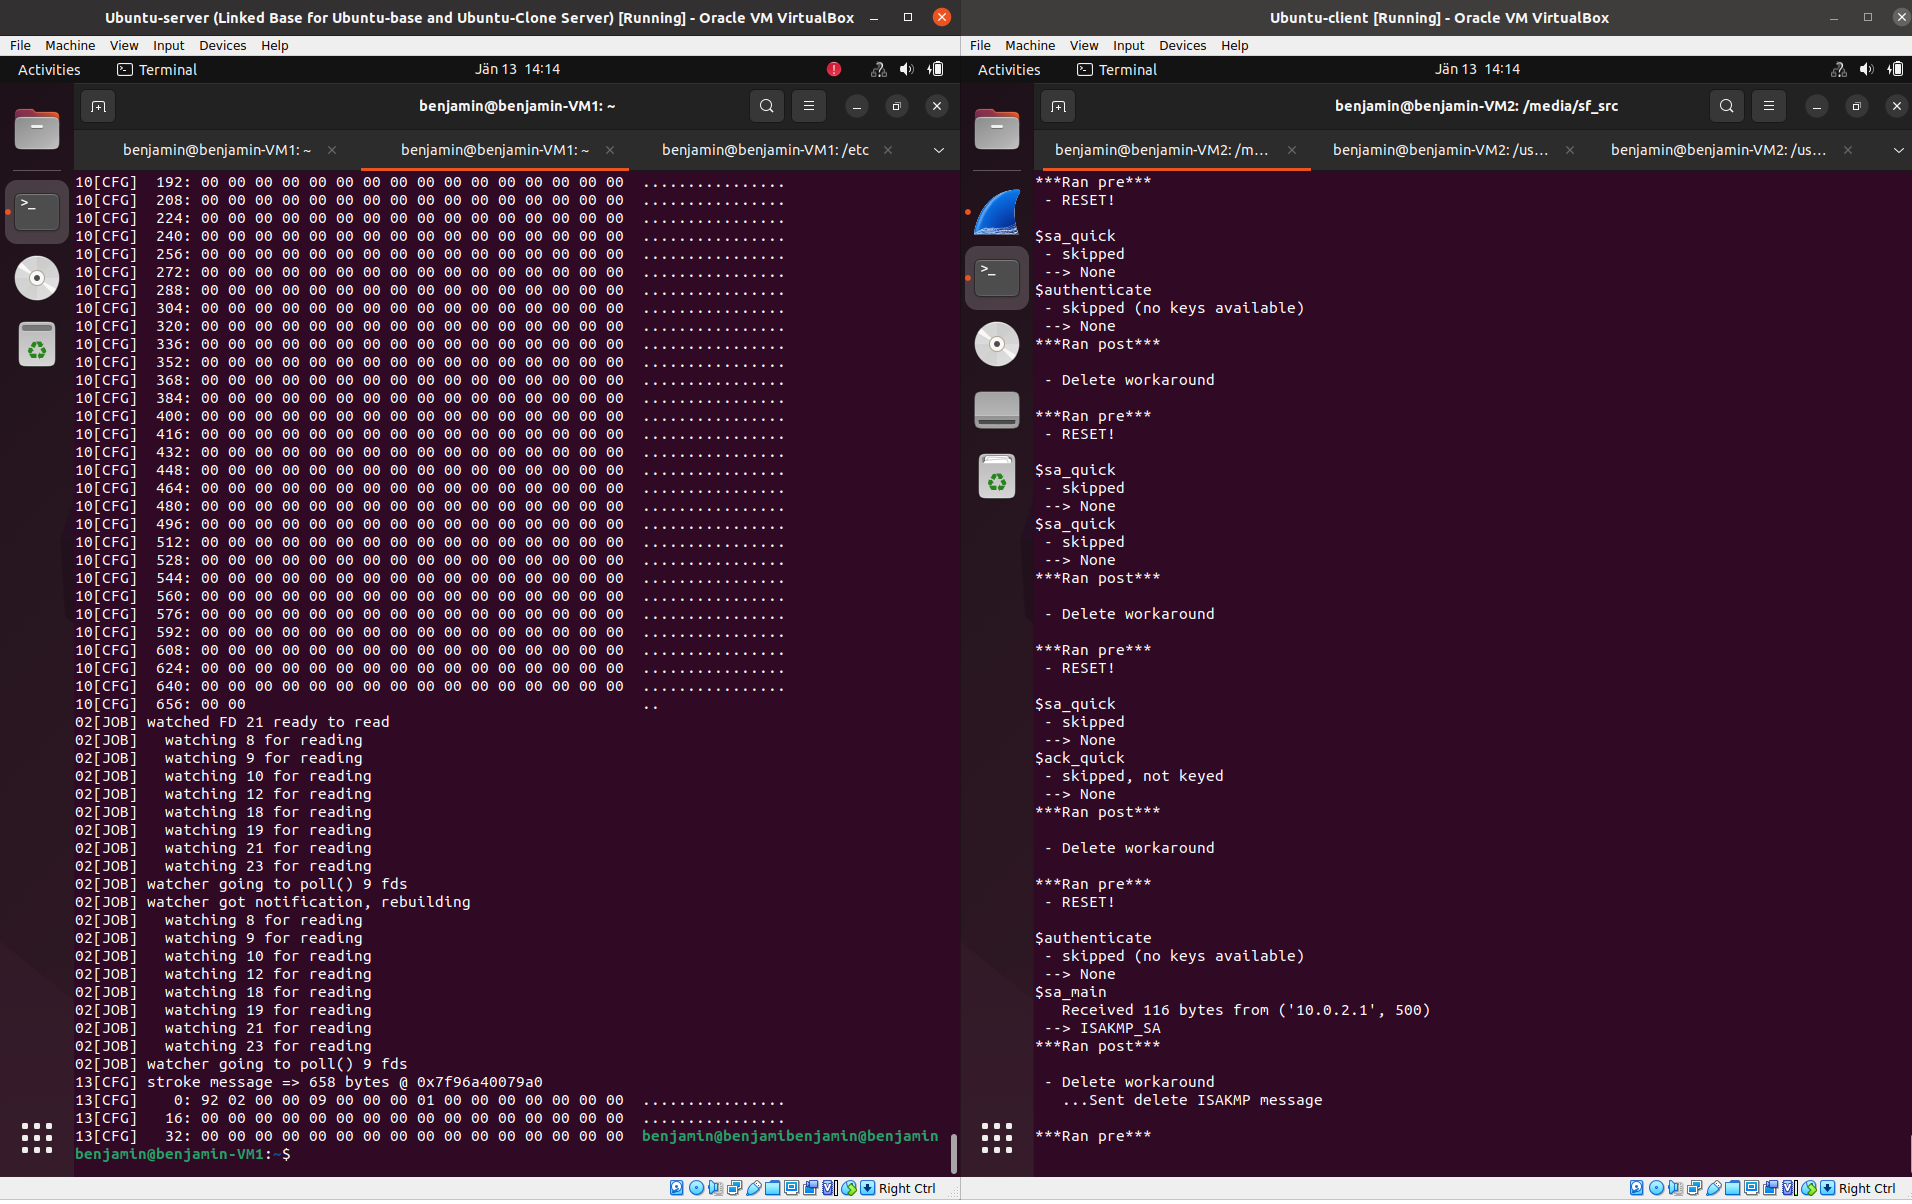
\includegraphics[width=\linewidth]{images/VM_setup}
	\caption{Pair of VMs running side by side, showing log output. \\Responder/server on the left, initiator/client on the right.}
	\label{fig:vmsetup}
\end{figure}


\section{VPN Configuration} \label{sec:vpn_setup}
The two \ac{ipsec} implementations learned and tested were strongSwan and Libreswan. Both are popular open source \ac{ipsec} implementations, with strongSwan featuring support for Linux, Android, FreeBSD, Apple OSX and Windows~\cite{doc:strongswan} and being the more widespread choice of the two. The libreswan \ac{ipsec} implementation supports Linux, FreeBSD and Apple OSX~\cite{doc:libreswan}. Both projects can trace their roots back to the now discontinued FreeS/WAN \ac{ipsec} project, an early \ac{ipsec} implementation for Linux. Both support \ac{ike}v1 and \ac{ike}v2, as well as an extensive list of additional features and authentication methods. For this project, we installed both implementations and configured them to use \ac{ike}v1 with \acp{psk} for authentication. The libreswan implementation uses a so-called \emph{ipsec.conf} configuration file to specify connection details including \ac{ike} version, mode and authentication type. The \ac{ipsec} background service is started/restarted via the commands \texttt{ipsec start} or \texttt{ipsec restart}. During learning and fuzzing, the \ac{ipsec} server was restarted before each execution of code, to ensure identical starting conditions.

The configuration file includes a setting to automatically ready the server connection and to wait for incoming connections on startup. On the other hand, strongSwan actually supports two types of configuration files. One more modern one using the Versatile IKE Control Interface (VICI), and another legacy option, also using an \emph{ipsec.conf} configuration file. The \ac{ipsec} service is started using the same commands. To make the configuration file translation between \ac{ipsec} implementations as straightforward as possible, we chose to use the \emph{ipsec.conf} configuration file for both implementations. What follows is an overview of the used \emph{ipsec.conf} settings for both implementations, as well as the full configuration files, shown in listings~\ref{lst:strongswan_config} and \ref{lst:libreswan_config}.

The \emph{ipsec.conf} settings control most facets of an \ac{ipsec} connection. The configuration consists of two major sections, \emph{config} and \emph{conn}. The \emph{config} section contains settings related to the general behavior of the \ac{ipsec} background service that is not limited to an individual connection. In our case, we specify the debugging behavior to log everything in Line~\ref{ln:strongswan_2} and set the \emph{uniqueids} setting to false in Line~\ref{ln:strongswan_3} of both configuration files. The \emph{uniqueids} setting is used to instruct the \ac{ipsec} implementations whether to treat individual IDs as globally unique or not. If set to ``no'', new exchanges with the same ID are applied to the existing connection instance instead of replacing it. We use this option, to ensure that we do not invalidate existing sessions with each subsequent \emph{ISAKMP SA} exchange and to not have the server ignore identical IDs. These settings apply to all connections configured in the configuration file.

\begin{lstlisting}[mathescape=true, float=ht, caption=strongSwan configuration, label=lst:strongswan_config]
	config setup $\label{ln:strongswan_1}$
		charondebug="all" $\label{ln:strongswan_2}$
		uniqueids=no $\label{ln:strongswan_3}$
	
	conn vm1tovm2 $\label{ln:strongswan_4}$
		auto=add $\label{ln:strongswan_5}$
		keyexchange=ikev1 $\label{ln:strongswan_6}$
		authby=secret $\label{ln:strongswan_7}$
		left=10.0.2.1 $\label{ln:strongswan_8}$
		leftsubnet=10.0.2.0/24 $\label{ln:strongswan_9}$
		right=10.0.2.2 $\label{ln:strongswan_10}$
		rightsubnet=10.0.2.0/24 $\label{ln:strongswan_11}$
		ike=aes256-sha1-modp2048! $\label{ln:strongswan_12}$
		esp=aes256-sha1! $\label{ln:strongswan_13}$
		ikelifetime=28800s $\label{ln:strongswan_14}$
		dpdaction=none $\label{ln:strongswan_15}$
		keyingtries=%forever $\label{ln:strongswan_16}$
\end{lstlisting}

Connection specific settings are configured in a \emph{conn} block and are given a name as an identifier, as seen in Line~\ref{ln:strongswan_4}. The \emph{auto} setting in Line~\ref{ln:strongswan_5} sets the default behavior when starting the \ac{ipsec} service. Setting it to ``add'' instructs the connection to be readied and to wait for incoming messages. This option allows us to bring the \ac{ipsec} server into a clean starting state by using either the \texttt{ipsec start} or \texttt{ipsec restart} console commands. Using the \emph{keyexchange} or 
\emph{ikev2} directives respectively in Line~\ref{ln:strongswan_6}, we specify that the communication will use the \ac{ike}v1 protocol. The \emph{authby} setting in Line~\ref{ln:strongswan_7} specifies the use of \acp{psk} for authentication. The next four following lines specify the involved IP ranges and subnets. The server or local IP is always referred to as the left side and the external connection partner is referred to as the right side of the \ac{ipsec} connection. Line~\ref{ln:strongswan_12} specifies the encryption/authentication algorithm to be used for the phase one (\ac{isakmp}) connection with the \emph{ike} keyword. The configured options are read as ``cipher-hashing algorithm-modgroup''. So in our case, the connections are configured to use \SI{256}{\bit} AES-CBC mode for encryption, SHA-1 as a hashing algorithm and the modp2048 Diffie-Hellman Group for key exchanges. Next follows the identical configuration for phase two (\ac{ipsec}) in Line~\ref{ln:strongswan_13}, with the \emph{esp} keyword. We use the same parameters here, as for the prior configuration, however, as keying information for phase two is generated in phase one, we no longer need the modgroup value. The \emph{ikelifetime} keyword in Line~\ref{ln:strongswan_14} determines how long the phase one connection will stay valid before the keys have to be replaced as a brute-force protection. ``dpdaction'' for strongSwan and ``dpddelay'' in combination with ``dpdtimeout'' for libreswan both serve to disable the \ac{dpd} feature of the \ac{ipsec} implementations. \ac{dpd} is a feature that allows \ac{ipsec} servers to probe the status of their connection peers in order to ensure their availability. As this creates additional traffic, we disable this feature for the testing environment. Finally, in Line~\ref{ln:strongswan_16} we allow unlimited keying attempts in order to allow for the efficient fuzzing of phase one messages.

\begin{lstlisting}[mathescape=true, float=ht, caption=libreswan configuration, label=lst:libreswan_config]
	config setup
		plutodebug=all
		uniqueids=no
	
	conn vm1tovm2
		auto=add
		ikev2=no
		authby=secret
		left=10.0.2.1 
		leftsubnet=10.0.2.0/24
		right=10.0.2.2
		rightsubnet=10.0.2.0/24
		ike=aes256-sha1-modp2048
		esp=aes256-sha1
		ikelifetime=28800s
		dpddelay=0
		dpdtimeout=0
		keyingtries=%forever
\end{lstlisting}

As can be seen in listings~\ref{lst:strongswan_config} and ~\ref{lst:libreswan_config}, the two configuration files only differ in a few lines. The main differences are in the debugging setting, as the two implementations use different management backends, and in how \ac{dpd} is disabled. Here, strongSwan has an explicit keyword to disable the function, while libreswan implicitly disables it if related settings are set to 0. Options not specified in the configuration file are set to their default values. Important default values relevant to the thesis include ``aggressive'', ``tunnel'' and ``pfs''. The ``aggressive'' keyword determines if \ac{ike} should run in \emph{Aggressive} mode or \emph{Main} mode, defaulting to Main mode. As Main mode is the more commonly used, as well as the more complicated option (including encryption), we leave this setting at its default value. The other two settings determine the type of \ac{vpn} connection to establish (defaults to tunnel mode) and the use of \ac{pfs} (defaults to \ac{pfs} enabled). Both are left at their default values. Starting the \ac{ipsec} server with the presented configuration options results in an easily-testable, basic \ac{vpn} setup.


\section{Debugging}
During any software development process, roughly 35-50 percent of development time is on the testing and validation of the software~\cite{britton2013reversible}. The development of our custom mapper and fuzzer required a very large amount of debugging, leaning more towards the 50 percent side of the aforementioned statistic. A common scenario was, that the mapper class would do some cryptographic calculations, but the server would return an error. Setting the debugging options in the respective configuration files to ``all'', has the \ac{ipsec} implementations log all internal procedures in great detail. This often gave more insight as to why specific packets were being rejected. However, in certain cases, a manual comparison of strongSwan-generated and our custom-generated \ac{ipsec} packets had to be performed on a byte-by-byte level. The open-source packet sniffing tool Wireshark~\cite{doc:wireshark} was used for this purpose. It allowed us to first connect the strongSwan client and then our own mapper class, all the while recording the traffic. This aided greatly in finding packet-level differences between the two implementations, allowing us to find and fix several bugs in ours. Unfortunately for debugging, \ac{ipsec}, or \ac{ike} to be more specific, encrypts large portions of its communication (everything past the first key exchange). This of course made analyzing the packets impossible, as the relevant information would be encrypted. Luckily, strongSwan allows for the logging of encryption keys and connection cookies. However, this setting is disabled by default. To enable it, one has to edit a different configuration file, namely the \emph{strongswan.conf} file, found usually in the same folder as the \emph{ipsec.conf} file. This other configuration file controls \ac{ipsec} management backend specific options, including a logging level. Setting this level to the highest (four), causes cryptographic keys to also be logged. An excerpt of the relevant log file can be seen in Figure~\ref{fig:keymateriallog}, where one can see the shared Diffie-Hellman secret, as well as all relevant keying material. The actual key used for the encryption of messages is denoted as the \emph{encryption key Ka}. The encryption key is generated by concatenating two hashes of the \emph{SKEYID\_e} and trimming to \SI{32}{\byte} (for AES-CBC-256 encryption). 

\begin{figure}
	\centering
	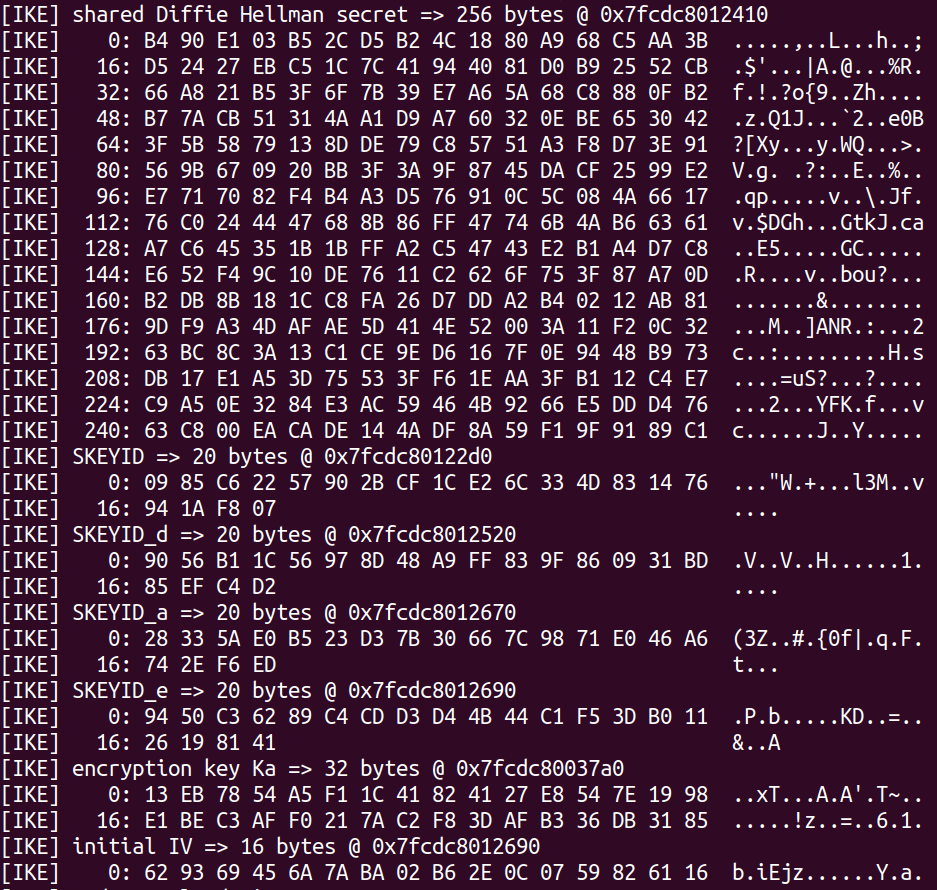
\includegraphics[width=0.7\linewidth]{images/key_material_log}
	\caption{\ac{ipsec} log excerpt showing keying information.}
	\label{fig:keymateriallog}
\end{figure}


Using the encryption key as well as the cookie of an \ac{ike} connection, the packets can be decrypted in Wireshark, by inputting the values in the corresponding protocol options field, as shown in Figure~\ref{fig:wiresharkdecryption}. Similar cryptographic information can be found in libreswan using the \texttt{ip xfrm state} command. The use of Wireshark for packet-level debugging greatly aided in the development of the custom mapper especially, as oftentimes, the relevant RFC specifications were rather unclear / left open to interpretation. A Wireshark packet dump of a sample \ac{ipsec} connection establishment between two strongSwan participants, as well as the corresponding decryption key and cookies is provided as supplementary material \TODO{supl}. Fortunately, all the effort invested into debugging our implementation resulted in a very detailed logging and testing toolkit for all parts of the implemented protocol. Additionally, once completed, the mapper class greatly reduced the time needed for further testing and fuzzing of the \ac{ipsec} servers, due to their flexible implementation.

\begin{figure}
	\centering
	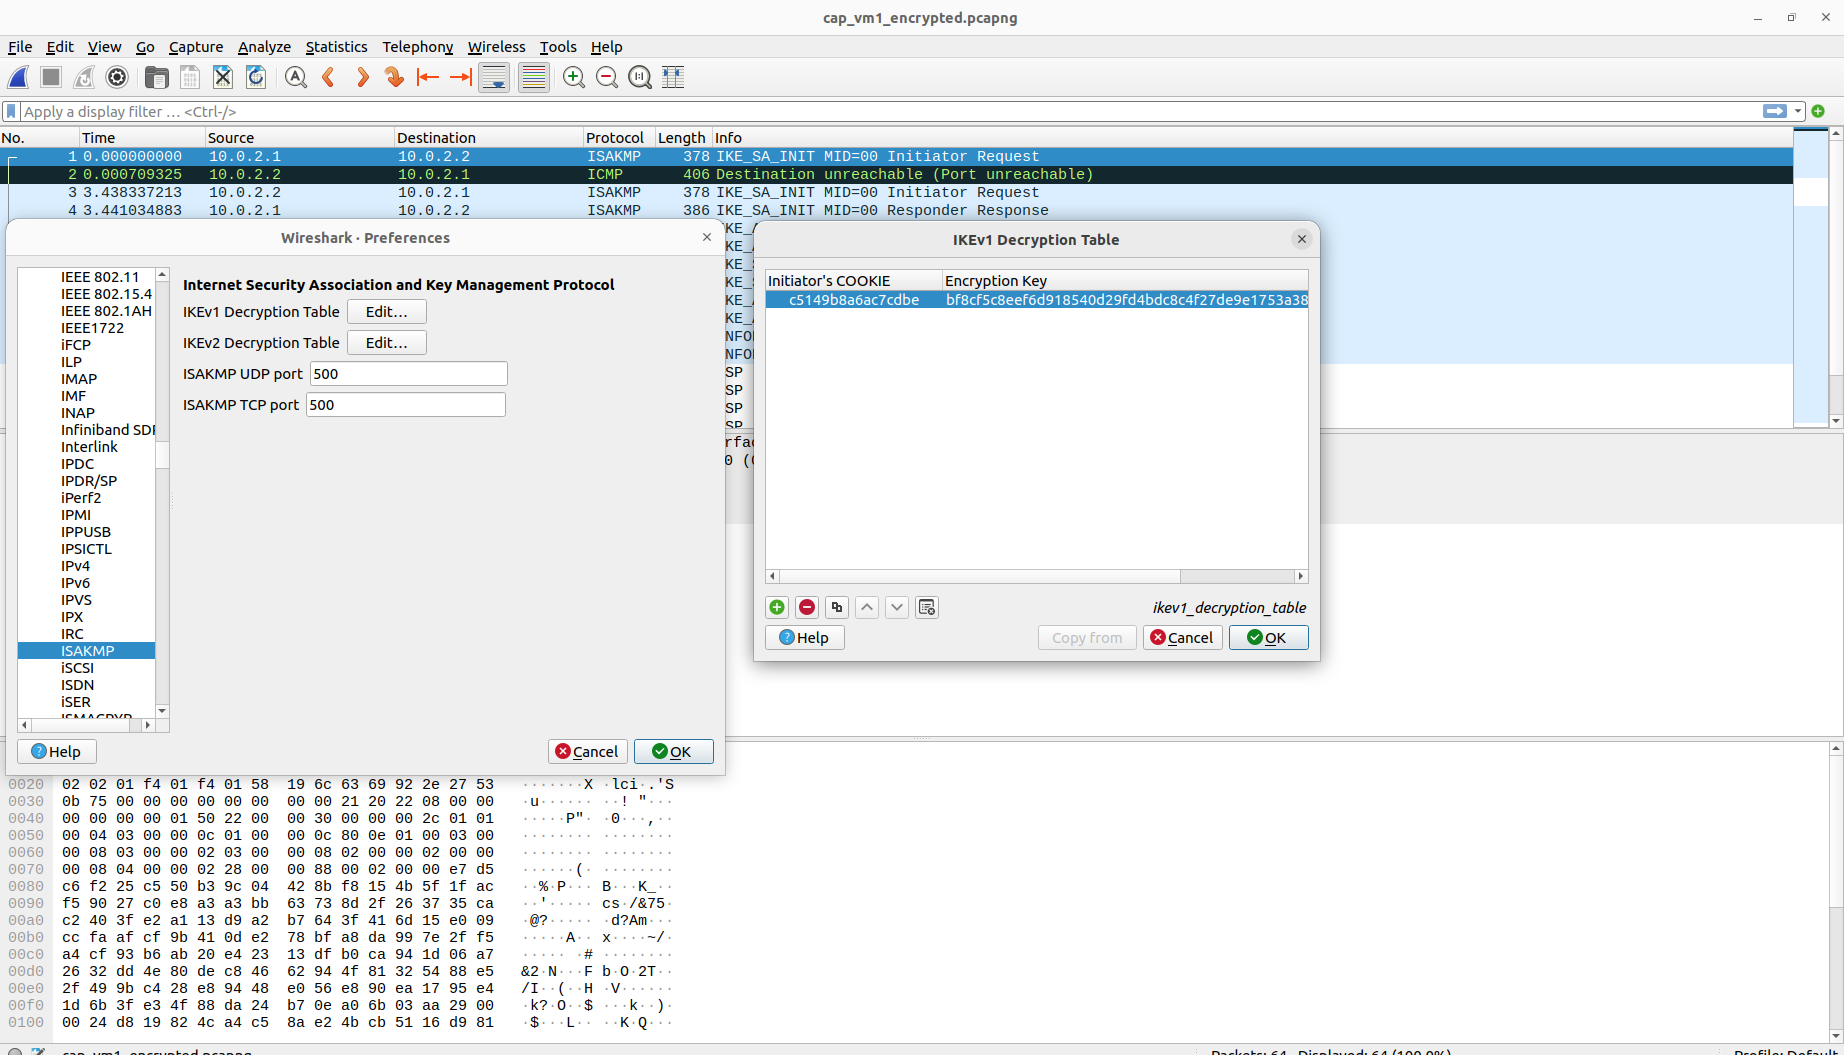
\includegraphics[width=\linewidth]{images/wireshark_decryption}
	\caption{Decrypting \ac{ipsec} packets in Wireshark.}
	\label{fig:wiresharkdecryption}
\end{figure}

